% !TEX TS-program = xelatex
% !TEX encoding = UTF-8 Unicode

% GSET Summer 2021 - Tennessee Technological University
% Tristan Hill - June 11, 2021
% Challenge 5 - Ascii Art Looping Challenge

\documentclass[12pt]{article}

% Custom Preamble
\usepackage{/home/thill/Documents/lectures/cpp_workshop/modules/cpp_tutorial} 

% Title and Misc
\newcommand{\MNUM}{8} %Module Number
\newcommand{\MNAME}{Introduction to C++} %Module Name
\newcommand{\TNAME}{ASCII Art} %Tutorial Name
\pagestyle{myheadings}
\markright{{\large GSET - Programming with Mr. Hill}}

\begin{document}

\thispagestyle{plain}

\begin{center}
   {\bf \large GSET - Programming with Mr. Hill - Summer 2021} \vspace{5mm}\\
   {\bf \Large \MNAME \hspc -  Challenge \hspc\MNUM\hspc - \TNAME}\vspace{3mm}\\
   
\end{center}

 %\hspace*{3cm}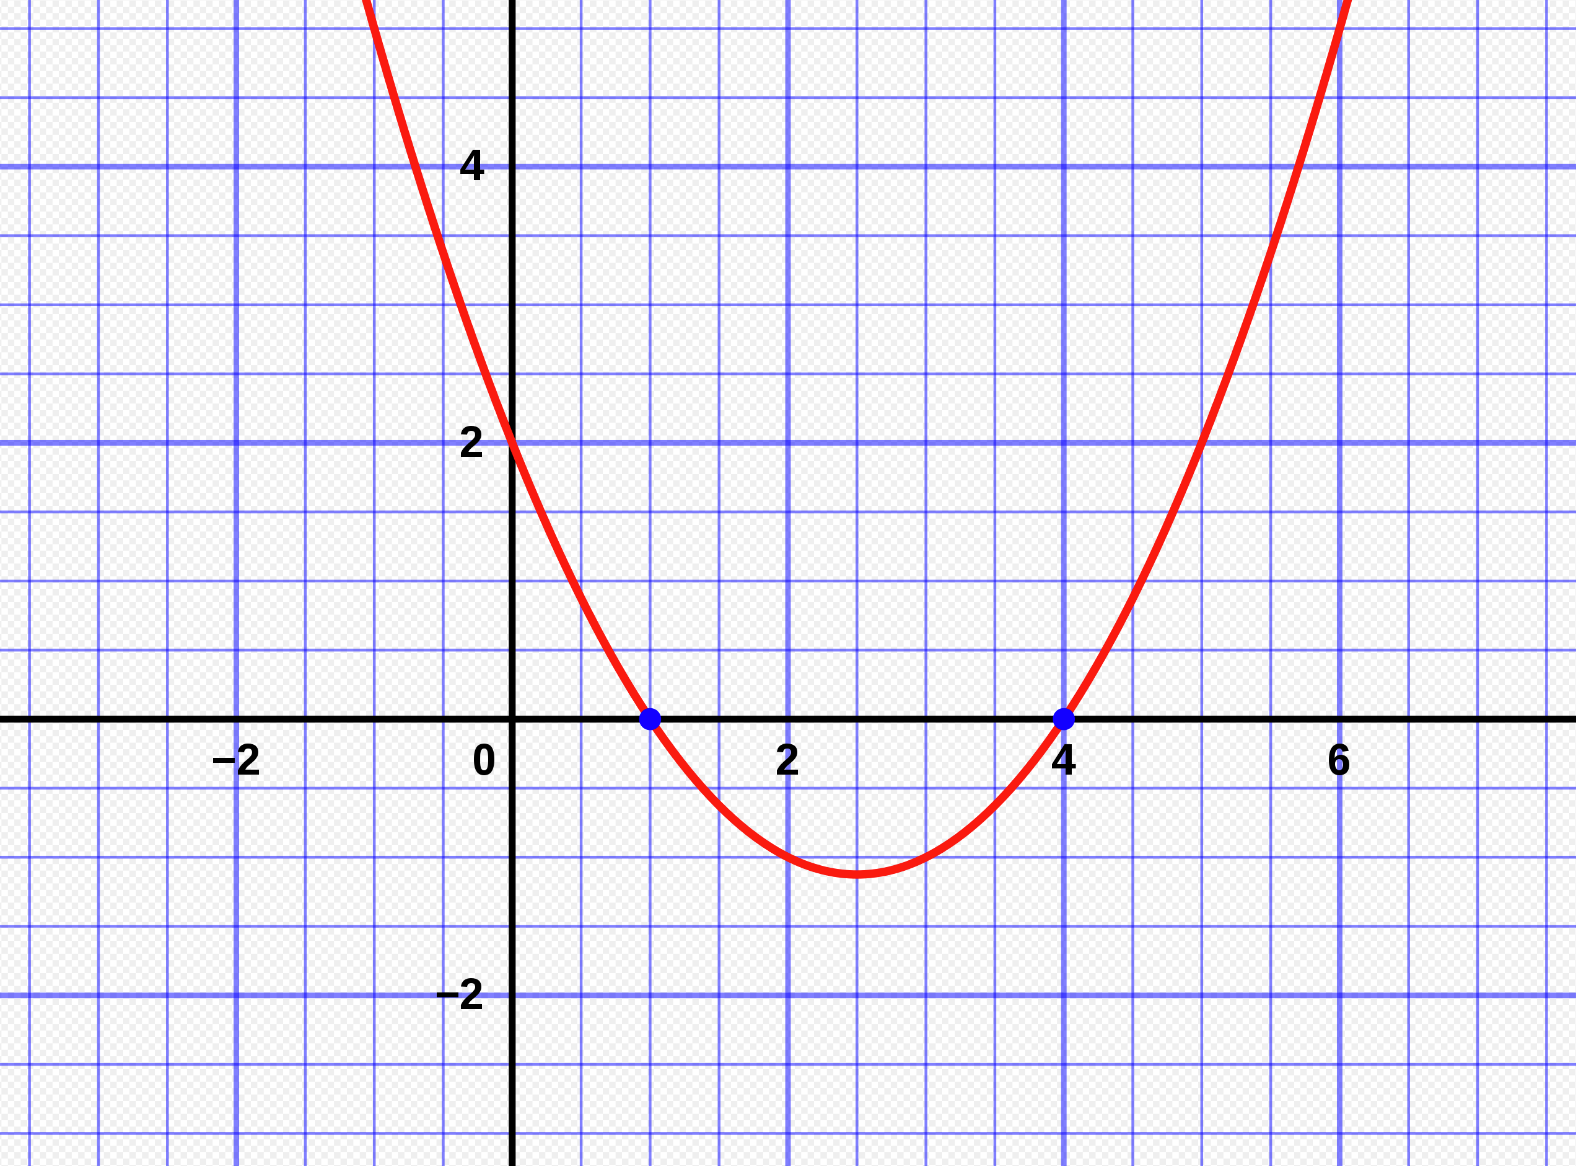
\includegraphics[scale=.15]{quad_equ.png} 

\begin{description}[labelindent=1cm]
	
	\item[\textbf{\underline{Overview:}}] \hfill \vspace{3mm}\\
	We are going to participate in the annual GSET ASCII art looping challenge! \vspace{5mm}\\
	
	\item[\textbf{\underline{ASCII art:}}] What is it? Awesome. \hfill \vspace{0mm}
	
	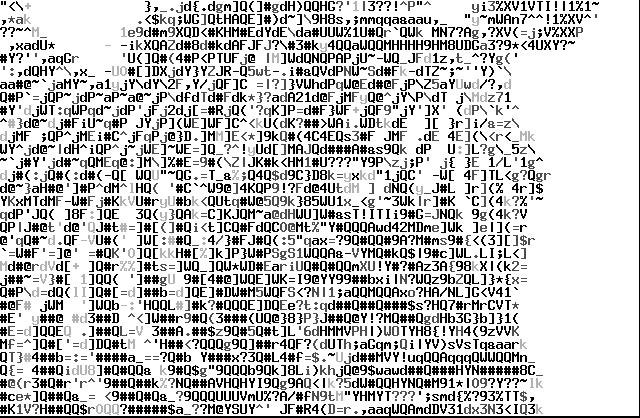
\includegraphics[scale=.3]{ascii_zebra_white}
	
\includegraphics[scale=.7]{ascii_r2d2}
	
	
	\item[\textbf{\underline{System Requirements:}}] \hfill \vspace{0mm}

\begin{itemize}
	\item {\bf Computer}: A computer is required to complete this tutorial. Any OS should work.
	\item {\bf MCU or PC:} This exercise can be completed with MCU or a desktop programming environment. If you use an MCU, print the art to the {\it serial monitor} or other serial terminal. If you use a desktop programming environment, print the art to the available terminal.
	
	\item {\bf C++:} You can use the online C++ compiler (\href{https://www.onlinegdb.com/online\_c++\_compiler}{OnlineGDB} ) or a C++ compiler of your choice.
\end{itemize}

	\item[\textbf{\underline{Problem Statement:}}] \hfill \vspace{0mm} \\
	Complete as many levels as possible by writing a C++ program to generate each of the images shown. 
	
	Note: Complete the levels in any order. If get stuck, move on to a different level. Also, each page contains a new type of challenges. If you are bored or stuck, you can move to the next page of levels.  
	
\newpage	
	
	\item[\textbf{\underline{The Levels:}}] \hfill \vspace{0mm} \\
	\begin{itemize}

		\item Level 0: The Line
		
		\begin{lstlisting}
		
		oooooooooooooooooooooooooooooooooooooooooooooooooo
		
		\end{lstlisting}
		
		\item Level 1: The Dotted Line
		
		\begin{lstlisting}
		
		 o o o o o o o o o o o o o o o o o o o o o o o o o
		
		\end{lstlisting}
		
		\item Level 2: The Dash-Dotted Line
		
		\begin{lstlisting}
		
		o--o--o--o--o--o--o--o--o--o--o--o--o--o--o--o--o-
		
		\end{lstlisting}
		
		\item Level 3: The Dash-Dotted-Asterisk Line
		
		\begin{lstlisting}
		
		*o-o-o*o-o-o*o-o-o*o-o-o*o-o-o*o-o-o*o-o-o*o-o-o*o
		
		\end{lstlisting}
		
		\newpage
		\item Level 4: The Rectangle
		
		\begin{lstlisting}
		
		oooooooooooooooooooo
		oooooooooooooooooooo
		oooooooooooooooooooo
		oooooooooooooooooooo
		oooooooooooooooooooo
		oooooooooooooooooooo
		oooooooooooooooooooo
		oooooooooooooooooooo
		oooooooooooooooooooo
		oooooooooooooooooooo
		
		\end{lstlisting}
		
		\item Level 5: The Stripes
		
		\begin{lstlisting}
		
		xxxxxxxxxxxxxxxxxxxxxxxxxxxxxxxxxxxxxxxxxxxxxxxxxx
		oooooooooooooooooooooooooooooooooooooooooooooooooo
		xxxxxxxxxxxxxxxxxxxxxxxxxxxxxxxxxxxxxxxxxxxxxxxxxx
		oooooooooooooooooooooooooooooooooooooooooooooooooo
		xxxxxxxxxxxxxxxxxxxxxxxxxxxxxxxxxxxxxxxxxxxxxxxxxx
		oooooooooooooooooooooooooooooooooooooooooooooooooo
		xxxxxxxxxxxxxxxxxxxxxxxxxxxxxxxxxxxxxxxxxxxxxxxxxx
		oooooooooooooooooooooooooooooooooooooooooooooooooo
		xxxxxxxxxxxxxxxxxxxxxxxxxxxxxxxxxxxxxxxxxxxxxxxxxx
		oooooooooooooooooooooooooooooooooooooooooooooooooo
		
		\end{lstlisting}
		
	    \item Level 6: The Grid
		
		\begin{lstlisting}
		
		ooooooooooooooooooooooooooooooooooooooooooooooooooo
		oxxxxoxxxxoxxxxoxxxxoxxxxoxxxxoxxxxoxxxxoxxxxoxxxxo
		oxxxxoxxxxoxxxxoxxxxoxxxxoxxxxoxxxxoxxxxoxxxxoxxxxo
		oxxxxoxxxxoxxxxoxxxxoxxxxoxxxxoxxxxoxxxxoxxxxoxxxxo
		oxxxxoxxxxoxxxxoxxxxoxxxxoxxxxoxxxxoxxxxoxxxxoxxxxo
		ooooooooooooooooooooooooooooooooooooooooooooooooooo
		oxxxxoxxxxoxxxxoxxxxoxxxxoxxxxoxxxxoxxxxoxxxxoxxxxo
		oxxxxoxxxxoxxxxoxxxxoxxxxoxxxxoxxxxoxxxxoxxxxoxxxxo
		oxxxxoxxxxoxxxxoxxxxoxxxxoxxxxoxxxxoxxxxoxxxxoxxxxo
		oxxxxoxxxxoxxxxoxxxxoxxxxoxxxxoxxxxoxxxxoxxxxoxxxxo
		ooooooooooooooooooooooooooooooooooooooooooooooooooo
		
		\end{lstlisting}
		
	\newpage
		
		\item Level 7: The Triangle
		
		\begin{lstlisting}
		
		x
		xx
		xxx
		xxxx
		xxxxx
		xxxxxx
		xxxxxxx
		xxxxxxxx
		xxxxxxxxx
		xxxxxxxxxx
		
		\end{lstlisting}
		
		\item Level 8: The Inverted Triangle
		
		\begin{lstlisting}
		
		xxxxxxxxxx
		xxxxxxxxx
		xxxxxxxx
		xxxxxxx
		xxxxxx
		xxxxx
		xxxx
		xxx
		xx
		x
		
		\end{lstlisting}
		
		\item Level 9: The Pyramid
		
		\begin{lstlisting}
		
		     x 
		    xxx
		   xxxxx
		  xxxxxxx
		 xxxxxxxxx
		xxxxxxxxxxx
		
		\end{lstlisting}
		 
	\end{itemize}

	{\bf If you you completed all 10 levels you can create your own level and challenge yourself or one of your peers. }
	

\newpage
\item[\textbf{\underline{Program Minimum Requirements:}}] \hfill \vspace{0mm}

The program should accomplish the following tasks. 

\begin{itemize}

	\item The ASCII art should be printed to the terminal window using a C++ program.

	\item The use of while loops or for loops is encouraged. Hardcoding the images into the program is discouraged.
	
\end{itemize}

\item[\textbf{\underline{Program Additional Requirements:}}] \hfill \vspace{0mm}

The program should accomplish the following tasks. 

\begin{itemize}
	
	\item The source of the image should be an .png file. Use OpenCV or other to load a .png file into your program. 
	
	\item An ASCII art version of the image should be printed to the terminal window using the C++ program.

	
\end{itemize}

\newpage

%\item[\textbf{\underline{Example Code:}}] \hfill \vspace{0mm}
%\begin{enumerate}
%    \item This is the C style way to output text.
%	%\begin{minted}{cpp}
%	\begin{lstlisting}
%
%// Arrays of Characters - GSET - Summer 2021 
%	
%#include <iostream>
%
%using namespace std;
%
%int main()
%{
%
%	char myname[]={"Tristan"};
%	
%	char c = 'T';
%	
%	cout<<"Hello World\n";
%	
%	cout<<myname<<endl; 
%	
%	cout<<myname[1]<<endl;
%	
%	cout<<(int)c<<"\a" <<endl; 
%	
%	return 0;
%}
%
%
%	\end{lstlisting}
%	%\end{minted}
%		
%\end{enumerate}

	\item[\textbf{\underline{Part 3 - Testing:}}] \hfill \vspace{0mm}
	\begin{enumerate}
	
		\item Complete the C++ code to the solve the problem described. \\\\
		
		\item Test your code with different inputs. Is the answer correct? How do you know? Are there certain inputs that do not work? \\\\
		
	
		\item Save your code with the download button or use copy and paste. You can view and edit the code in any text editor. Also, save a copy of the program output for your tutorial summary. \\\\

	\end{enumerate}

\newpage
\item[\textbf{\underline{Solution Code:}}] \hfill \vspace{0mm}
%
%\begin{lstlisting}
%
%\end{lstlisting}
%
%\item[\textbf{\underline{Tutorial Complete:}}] \hfill \vspace{3mm}\\ 
%	Congratulations, after completing {\it Tutorial 2 - Quadratic Equation}, you have begun learning to program in C++! You are now ready to start learning about more complex data structures and program flow. \\
%

\newpage
\item[\textbf{\underline{Tutorial Summary:}}] \hfill \vspace{3mm}\\ 

A summary is not required for this challenge.

\item[\textbf{\underline{Submission on Teams:}}] \hfill \vspace{3mm}\\ 
Use the appropriate shared folder on Teams to submit your program and summary. Submit the fol1owing items with your TNTech username in the filenames as shown below. \vspace{0mm}\\

\underline{Files for Tutorial 1 (TNTech Username : twhill21)}

\begin{itemize}

%\item Tutorial Summary: \textbf{ twhill21\_summary2.txt}

\item C++ Source Code: \textbf{ twhill21\_challenge8.cpp}

\end{itemize}


\end{description}
\end{document}

